% Search for all the places that say "PUT SOMETHING HERE".


\documentclass[11pt]{article}
\usepackage{amsmath,textcomp,amssymb,geometry,graphicx}

\def\Name{Ben Augarten}  % Your name
\def\Var{\text{Var}}
\def\CoVar{\text{CoVar}}
\title{CS189--Spring 2013 --- Solutions to Homework 2}
\author{\Name}
\markboth{CS170--Spring 2012 Homework 2 \Name}{CS170--Spring 2012 Homework 2 \Name}
\pagestyle{myheadings}

\begin{document}
\maketitle

\begin{enumerate}
\item We want to pick a class, $j$ that minimizes:
$\sum\limits_{k}L_{kj}P(\omega_k|x)$, $L_{kj}$ being the loss incurred by choosing class $j$ when the actual class is $k$.\\
$L_{kj}=0$, if $k=j$\\
$L_{kj}=\lambda_d$, if $j$ is the $c+1$ class, the doubt class\\
$L_{kj}=\lambda_s$, otherwise\\

$\min(\lambda_sP(w_0|x)+\lambda_sP(w_1|x)+...+ 0*P(\omega_j|x) + ... + \lambda_sP(w_{c}|x), \lambda_d)$\\
When do we choose to make a decision?\\
$\lambda_sP(w_0|x)+\lambda_sP(w_1|x)+...+ 0*P(\omega_j|x) + ... + \lambda_sP(w_{c}|x) \le \lambda_d$\\
$\lambda_s(1-P(\omega_j|k)) \le \lambda_d$\\
$1-\frac{\lambda_d}{\lambda_s}\le P(\omega_j|k)$\\
And then, of course when we make a decision, we choose the best one, that is, all $\lambda_s$ being equal, we choose the maximum $P(\omega_k|x)$\\
Therefore, we decide $\omega_i$ if $P(\omega_i|x)>P(\omega_j|x)$ for all $j$ and $P(\omega_i|x)\ge 1-\frac{\lambda_d}{\lambda_s}$

\item
$p(x|w_i)\sim N(\mu_i, \sigma^2)$\\
$p(w_i|x)=p(x|w_i)p(w_i)$ normalized\\
$p(w_i|x)=\frac{1}{2}N(\mu_i, \sigma^2)$\\
Let $\mu_2 > \mu_1$. There exists some value for which we change our guess from $w_1$ to $w_2$. This value is equidistant from each of the means (this is intuitive from the symmetry in the problem because both have the same variance). We can also just set $N(\mu_1, \sigma^2)=N(\mu_2, \sigma^2)$ to find out that this value, $b$, is $\frac{\mu_2+\mu_1}{2}$. The probability of error is the probability of it being $w_2$ when $x<b$ and the probability of it being $w_1$ when $x>b$.\\
$\int\limits_{-\infty}^{b}P(w_2|x)P(x)dx + \int\limits_{b}^{\infty}P(w_1|x)P(x)dx$\\
Similarly, by symmetry, the two integrals are going to be equal (because both are normally distributed with same standard deviation).\\
$2*\int\limits_{b}^{\infty}\frac{1}{2\sigma\sqrt{2\pi}}\exp{\frac{-(x-\mu_1)^2}{2\sigma^2}}dx$\\
Now lets substitute variables, $u=\frac{x-\mu_1}{\sigma}$, $\sigma du=dx$, 
and then new bound is $\alpha = \frac{\mu_2-\mu_1}{2\sigma}$\\
$\int\limits_{\alpha}^{\infty}\frac{1}{\sqrt{2\pi}}\exp{-\frac{1}{2}u^2}du$\\
$\int\limits_{\alpha}^{\infty}\frac{1}{\sqrt{2\pi}}\exp{-\frac{1}{2}u^2}du\le \frac{1}{\sqrt{2\pi}a}e^{-(1/2)a^2}\\
P_e\le\lim\limits_{a\to \infty}\frac{1}{\sqrt{2\pi}a}e^{-(1/2)a^2}=0\\
$
\item Let Y be the discrete r.v. corresponding to score of a shot \\
$E(Y)=4*P(Y=4)+3*P(Y=3)+2*P(Y=2)+0$\\
$E(Y)=4*P(X\le \frac{1}{\sqrt{3}})+3*P(\frac{1}{\sqrt{3}}\le X\le 1)+2*P(1\le X\le \sqrt{3})$\\
$E(Y)=4*\int\limits_{0}^{\frac{1}{\sqrt{3}}}f(x)dx+3*\int\limits_{\frac{1}{\sqrt{3}}}^{1}f(x)dx+2*\int\limits_{1}^{\sqrt{3}}f(x)dx$\\
$E(Y)=4*\frac{1}{3}+3*\frac{1}{6}+2*\frac{1}{6}$\\
$E(Y)=13/6\approx 2.167$

\item
$f(x,y)=x+y\\
g(x)=\int\limits_{0}^{1}(x+y)dy\\
g(x)=\left. xy+\frac{1}{2}y^2 \right|_{y=0}^{1}\\
g(x)=x+\frac{1}{2}\\
E(X)=\int\limits_0^1 xg(x)dx\\
E(X)=\int\limits_0^1 x^2+\frac{1}{2}xdx\\
E(X)=\left. \frac{1}{3}x^3+\frac{1}{4}x^2 \right|_{x=0}^1\\
E(X)=7/12\\
\Var(X)=E(X^2)-(7/12)^2\\
\Var(X)=\int\limits_0^1 x^2(x+\frac{1}{2})dx\\
\Var(X)=5/12\\\\
h(y)=\int\limits_{0}^{1}(x+y)dx\\
h(y)=y+\frac{1}{2}\\
E(Y)=\int\limits_0^1 y^2+\frac{1}{2}ydy\\
E(Y)=7/12\\
\Var(Y)=\int\limits_0^1 y^2(y+\frac{1}{2})dy\\
\Var(Y)=5/12\\
\CoVar(X, Y)=E(XY)-(7/12)^2\\
\CoVar(X, Y)=\int\limits_0^1\int\limits_0^1 xy(x+y)dxdy - (7/12)^2\\
\CoVar(X,Y) = 1/3\\
$

\item
\begin{enumerate}
\item
The likelihood of of getting samples $x_1..x_n$, $L_n$ is equal to $p(x_1;\theta)p(x_2;\theta)..p(x_n;\theta)$\\
As long as $\theta > x_i$, $p(x_i;\theta)=\frac{1}{\theta}$\\
$L_n=\left( \frac{1}{\theta} \right)^n$\\
if $\max(x_1,x_2,..,x_n) > \theta$, then there will be a zero probability and $L_n=0$\\
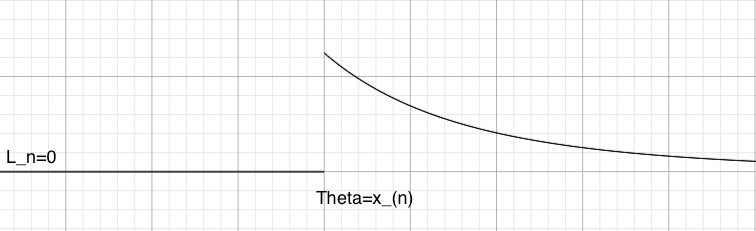
\includegraphics[width=5.5in]{p5_graph.png}
\item
$x_{(n)}$ is the maximum likelihood estimate -- $\theta=x_{(n)}$ maximizes $L_n$, and is therefore the most likely value of $theta$ given the observations $x_1,..,x_n$.
\item
Our estimate is most likely not the expected value of $\theta$. If we have a reading of $x_n$ then it is likely that $\theta$ is larger than $x_n$. Therefore, our estimate is biased.
\end{enumerate}
\item
$\log L(\theta)=\log\prod\limits_{i}\theta e^{-\theta x_i}$\\
$\log L(\theta)=\sum\limits_i \log\theta e^{-\theta x_i}$\\
$\log L(\theta)=\sum\limits_i \log\theta -\theta x_i$\\
$\frac{dL(\theta)}{d\theta}=\sum\limits_i \frac{1}{\theta}-x_i=0$\\
$\frac{5}{\theta}=(x_1+x_2+..+x_5)=5.7$\\
$\theta = .877$\\
$\frac{d^2L(\theta)}{d\theta^2e}= -\sum\limits_i \frac{1}{\theta^2}<0$\\
$\theta = .877$

\item Let $x_m$ be the middle $x$ value, for which we change our guess (there shouldn't be more than one)\\
$P(\omega_1|x)=P(x|\omega_1)P(\omega_1)\\
P(\omega_1|x)=\frac{1}{2}e^{-\lambda_1}\frac{\lambda_1^x}{x!}\\
P(\omega_2|x)=\frac{1}{2}e^{-\lambda_2}\frac{\lambda_2^x}{x!}\\
P(\omega_1|x_m)=P(\omega_2|x_m)\\
e^{-\lambda_1}\frac{\lambda_1^{x_m}}{x_m!}=e^{-\lambda_2}\frac{\lambda_2^{x_m}}{x_m!}\\
-\lambda_1+x_m\ln(\lambda_1)=-\lambda_2+x_m\ln(\lambda_2)\\
x_m(\ln(\lambda_1)-\ln(\lambda_2))=-\lambda_2+\lambda_1\\
x_m=\frac{\lambda_2-\lambda_1}{\ln(\lambda_2)-\ln(\lambda_1)}=12.33\\
$
For $x<x_m$, we pick the lower value of $\lambda$, lets say $\lambda_1$. For $x\ge x_m$ we pick $\lambda_2$\\
Probability of correct classification for $\omega_1$ is\\
$\sum\limits_{0}^{\lfloor x_m\rfloor}P(\omega_1,x)$\\
$\sum\limits_{0}^{12}\frac{1}{2}e^{-10}\frac{10^x}{x!}$\\
Probability of correct classification for $\omega_1$ is $39.6$\%\\
$\sum\limits_{13}^{\infty}\frac{1}{2}e^{-15}\frac{15^x}{x!}$\\
Probability of correct classification if its of class $\omega_2$ is $36.6$\%\\
Probability of error:\\
$P(error)=\sum\limits_{0}^{12}P(\omega_2,x)+\sum\limits_{13}^{\infty}P(\omega_1,x)$\\
$P(error)=\sum\limits_{0}^{12}\frac{1}{2}e^{-15}\frac{15^x}{x!}+\sum\limits_{13}^{\infty}\frac{1}{2}e^{-10}\frac{10^x}{x!}\\
=.24\\
$
\\
Now lets do it using two independent trials.
Let $y=x_1+x_2$\\
$P(y|\omega_1)\sim Poisson(2\omega_1)\\
P(y|\omega_2)\sim Poisson(2\omega_2)\\
P(\omega_1|y)=\frac{1}{2}e^{-2\lambda_1}\frac{(2\lambda_1)^x}{x!}\\
P(\omega_2|y)=\frac{1}{2}e^{-2\lambda_2}\frac{(2\lambda_2)^x}{x!}\\
P(\omega_1|y)=P(\omega_2|y)\\
-2\lambda_1+y_m\ln(2\lambda_1)=-2\lambda_2+y_m\ln(2\lambda_2)\\
y_m=\frac{2(\lambda_2-\lambda_1)}{\ln(2\lambda_2)-\ln(2\lambda_1)}\\
y_m=24.66\\
$
Probability of correct classification for $\omega_1$\\
$
\sum\limits_0^{\lfloor y_m \rfloor}\frac{1}{2}e^{-2\lambda_1}\frac{(2\lambda_1)^x}{x!}\\
=42.2\%\\
$
Probability of correct classification for $\omega_2$\\
$
\sum\limits_{\lceil y_m \rceil}^{\infty}\frac{1}{2}e^{-2\lambda_2}\frac{(2\lambda_2)^x}{x!}\\
=42.1\%\\
$
$P(error)=\sum\limits_{0}^{24}P(\omega_2,y)+\sum\limits_{25}^{\infty}P(\omega_1,y)$\\
$P(error)=\sum\limits_{0}^{24}\frac{1}{2}e^{-30}\frac{30^x}{x!}+\sum\limits_{25}^{\infty}\frac{1}{2}e^{-20}\frac{20^x}{x!}\\
=15.7\%\\
$




\end{enumerate}
\end{document}
